\documentclass{beamer}

\mode<presentation> {
\usetheme[secheader]{Madrid}
\usecolortheme{seahorse}
\useinnertheme{circles}
}

\usepackage{graphicx} % Allows including images
\usepackage{booktabs} % Allows the use of \toprule, \midrule and \bottomrule in tables
\usepackage{tikz}
\usepackage{caption}
\usepackage{hyperref}



%----------------------------------------------------------------------------------------
%	TITLE PAGE
%----------------------------------------------------------------------------------------

\title[History of HCI]{History of HCI} % The short title appears at the bottom of every slide, the full title is only on the title page

\author{Chaklam Silpasuwanchai} % Your name
\institute[AIT] % Your institution as it will appear on the bottom of every slide, may be shorthand to save space
{
Asian Institute of Technology \\ % Your institution for the title page
\medskip
\textit{chaklam@ait.asia} % Your email address
}
\date{} % Date, can be changed to a custom date

\AtBeginSection[]
{
\begin{frame}<beamer> 
\tableofcontents[currentsection]  % show TOC and highlight current section
\end{frame}
}

\begin{document}

\begin{frame}
\titlepage % Print the title page as the first slide
\end{frame}

%\begin{frame}
%	\frametitle{Reminder} % Table of contents slide, comment this block out to remove it
%	\begin{itemize}
%		\item Phase 0: Team forming due soon
%	\end{itemize}
%\end{frame}

\begin{frame}
\frametitle{Overview} % Table of contents slide, comment this block out to remove it
\tableofcontents % Throughout your presentation, if you choose to use \section{} and \subsection{} commands, these will automatically be printed on this slide as an overview of your presentation
\end{frame}

%----------------------------------------------------------------------------------------
%	PRESENTATION SLIDES
%----------------------------------------------------------------------------------------

\begin{frame}
\frametitle{Sources} 
\begin{itemize}
		\item Mackenzie, Chapter 1, \textbf{History Context}, Human Computer Interaction: An Empirical Research Perspective, 1st ed. (2013) 
		\item Shneiderman, \textbf{Direct Manipulation: A Step Beyond Programming Languages} (1983)
		\item Macintosh 128K, \url{https://en.wikipedia.org/wiki/Macintosh_128K}
\end{itemize}
\end{frame}


%------------------------------------------------
\section{Historical Context} % Sections can be created in order to organize your presentation into discrete blocks, all sections and subsections are automatically printed in the table of contents as an overview of the talk
%------------------------------------------------

\subsection{Introduction} % A subsection can be created just before a set of slides with a common theme to further break down your presentation into chunks


\begin{frame}
\frametitle{Early Days}
\begin{itemize}
	\item In 1940s, computers are too \textbf{precious}, too \textbf{complicated}
	\item Only selected scientists/engineers were allowed to access
	\begin{itemize}
		\item Most \textbf{non-user-friendly }tasks like \textit{grep that requires regular expression} or \textit{vi's editor that lack feedback when switching mode} is \textit{NOT} an issue, because these people are the one \textbf{who invent themselves}! 
%		\item Interactions was \textbf{not on the minds} of the engineers and scientists who designed, built, configured the early computers
	\end{itemize}
	\item But by 1980s, everything changes.  Computers become not only powerful, but \textbf{accessible by anyone!}  HCI becomes a very important aspect
\end{itemize}
\end{frame}

\begin{frame}
\frametitle{Interdisciplinary Nature of HCI}
\begin{itemize}
	\item HCI owes a lot to older disciplines
	\item The most central is \textit{human factors} or \textit{ergonomics}
	\begin{itemize}
		\item CHI ''human factors" named after
		\item Concerns \textbf{human capabilities}, \textbf{limitations}, and \textbf{performance} (but NOT user experience)
	\end{itemize}
	\item HCI evolves and becomes very broad in scope. 
	\begin{itemize}
	\item Draws interests from many disciplines - psychology, design, engineering, etc.
	\end{itemize}
\end{itemize}
\end{frame}

\begin{frame}
\frametitle{Notable events in the history of HCI}
	\begin{figure}
	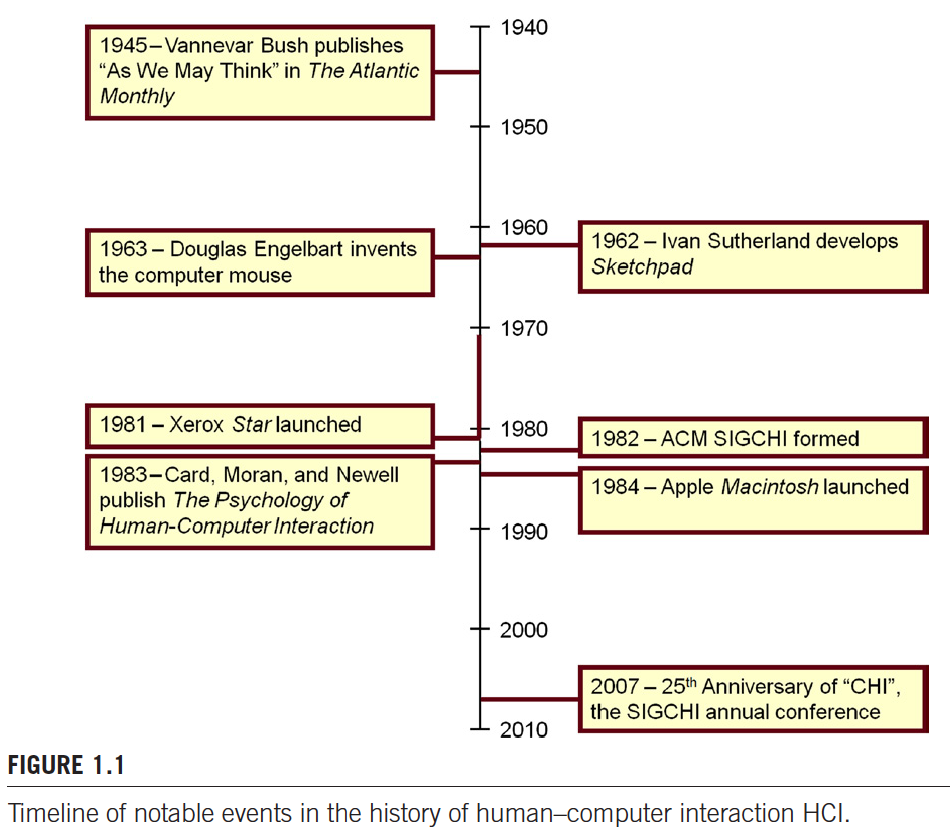
\includegraphics[width=0.6\linewidth]{timeline}
	\caption{Source: Fg 1.1 (Mackenzie)}
\end{figure}

\end{frame}

\subsection{Vannevar Bush's ``as we may think" (1945)} % A subsection can be created just before a set of slides with a common theme to further break down your presentation into chunks


\begin{frame}
\frametitle{Who is Vannevar Bush}

\begin{columns}[c] % The "c" option specifies centered vertical alignment while the "t" option is used for top vertical alignment
	
	\column{.4\textwidth} % Left column and width
	\begin{figure}
			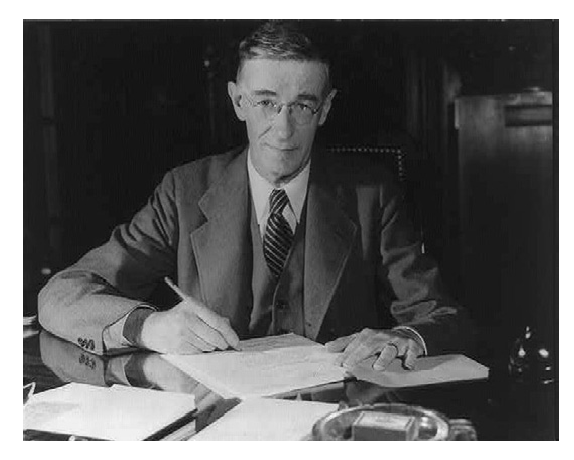
\includegraphics[width=1\linewidth]{bush}
			\caption{Source: Figure 1.2 (Mackenzie)}
	\end{figure}

	
	\column{.6\textwidth} % Right column and width
	\begin{itemize}
		\item Bush published a \textbf{prophetic essay} ``As We May Think" in Atlantic Monthly in July, 1945 (cited 4000+ times)
		\item Bush was U.S. government's Director of the Office of Scientific Research and scientific advisor to Roosevelt
		\item During WWII, he leads 6,000 scientists in the application of science to warfare
	\end{itemize}
	
\end{columns}
\end{frame}

\begin{frame}
\frametitle{Vannevar Bush's Essay (1945)}
	\begin{itemize}
%		\item His essay concerns the \textbf{dissemination}, \textbf{storage}, and \textbf{access} to scholarly knowledge
		\item Raises the problem of \textbf{information overload} and \textbf{difficulty} in accessing knowledge
		\item Proposes \textit{memex}, which contains a key concept of \textit{associative indexing} - selecting one item retrieves other relevant (sounds a lot like \textbf{hyperlink} today!)
		\item Beginning of many inspirations to follow (just like how \textit{Doraemon} inspires engineering culture in Japan)
	\end{itemize}
\end{frame}

\subsection{Ivan Sutherland's Sketchpad (1962)} % A subsection can be created just before a set of slides with a common theme to further break down your presentation into chunk
\begin{frame}
\frametitle{Ivan Sutherland's Sketchpad (1962)}
	\centering
	\begin{figure}
		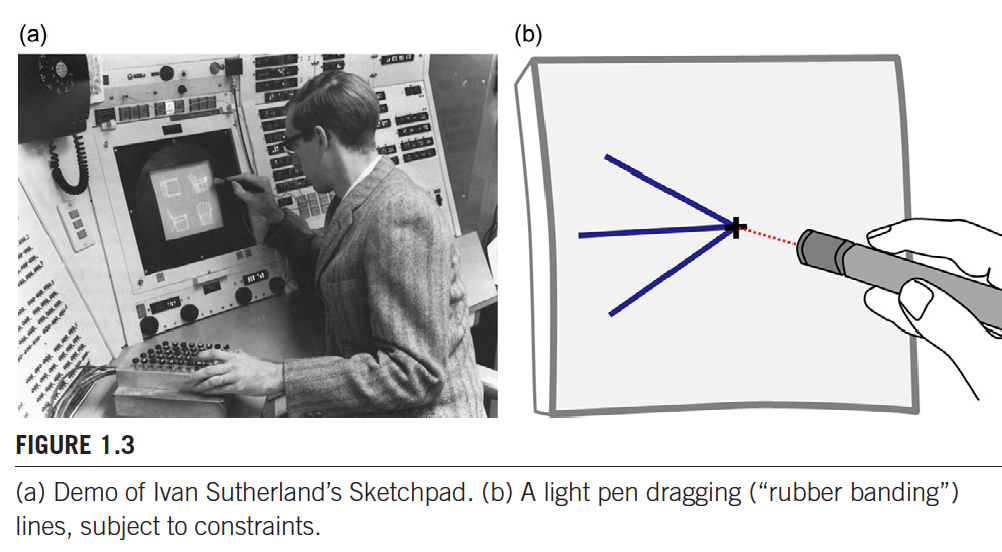
\includegraphics[width=0.5\linewidth]{ivan}
		\caption{Source: Fg 1.3 (Mackenzie)}
	\end{figure}
\begin{itemize}
	\item Developed \textit{Sketchpad} as part of his PhD research at MIT
	\item Sketchpad was a graphic system supported the \textbf{drawings} of shapes and lines using a l\textbf{ight pen}
%	\item Sketchpad was developed under the usability issues of commands that require expertise and cognitive effort
	\item \url{https://www.youtube.com/watch?v=YB3saviItTI}
\end{itemize}
\end{frame}

\begin{frame}
%\footnotesize
\frametitle{Direct Manipulation}
Sketchpad - the first \textit{direct manipulation} interface
\begin{itemize}
	\item \textbf{Visibility of objects} - continuous representations %of objects
	\item \textbf{Incremental action} - action such as mouse selection %that incrementally changing the state of the system
	\item \textbf{Rapid feedback} - immediate feedback %of the action where impact on the object of interest is immediately visible; users can check whether how far from their goal is
	\item \textbf{Reversibility} - can be easily undo %and users experience less anxiety in trying; error message is rarely needed
	\item \textbf{Exploration} - permits discovery and learning %process, and users gain confidence and mastery - novice to experts
	\item \textbf{Syntactic correctness of all actions} - menus and buttons %make sure the systems can limit users to only legal actions
	\item \textbf{Replacing language with action} - directly manipulating %the object of interests using pen, touch, or any other natural means, instead of typing language
\end{itemize} 
\end{frame}

\subsection{Invention of the Mouse (1963)} % A subsection can be created just before a set of slides with a common theme to further break down your presentation into chunks

\begin{frame}
\frametitle{Douglas Engelbart's mouse (1963)}
\begin{itemize}
	\item Mouse \textbf{symbolizes} the emergence of HCI
	\item Invented by Douglas Engelbart in 1963%, \textbf{fundamentally change} the way humans interact
	\item The light pen was not so usable as \textbf{user held the pen in the air which is tiring}. %Engelbart was working at Stanford Research Institute on an hypertext system called NLS. 
	\item Device besides the keyboard makes sense
\end{itemize}
\end{frame}


\begin{frame}
\frametitle{Engineering of the Mouse}
\centering
\begin{figure}
	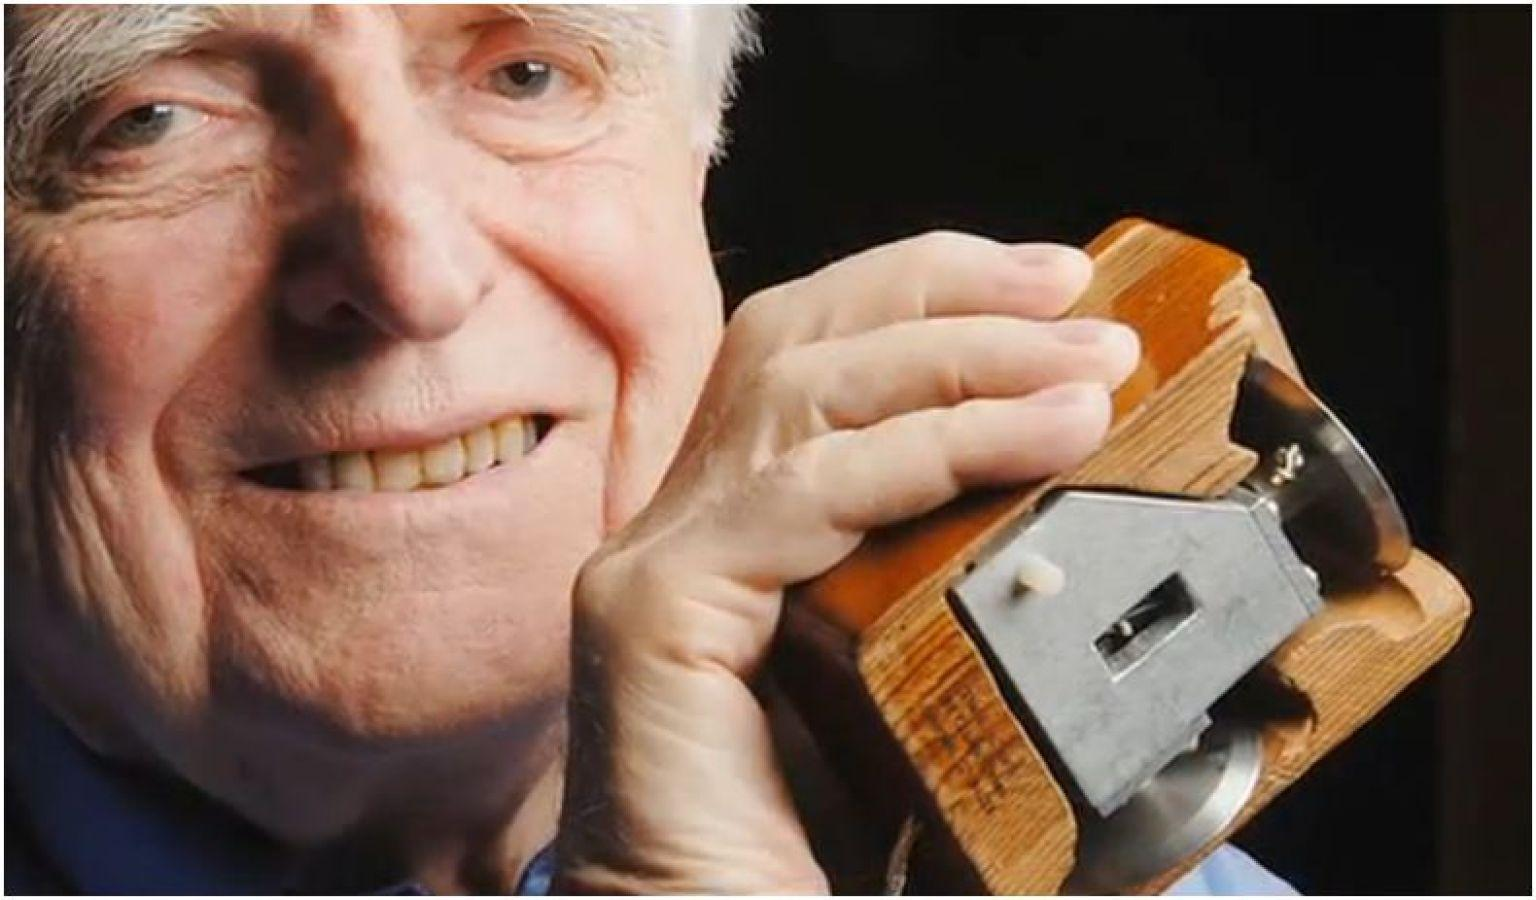
\includegraphics[width=0.65\linewidth]{mouse}
	\caption{Source: Fg 1.4 (Mackenzie)}
\end{figure}
\vspace{-10pt}
\begin{itemize}
	\item The first prototype included \textbf{one button} and \textbf{two wheels} positioned at right angles to each other, marking xy
	\item A selection button at the user's index finger.
	\item Later, Engelbart developed a three-button version
\end{itemize}
\end{frame}

\begin{frame}
\frametitle{HCI First User Study}
\centering
\begin{figure}
	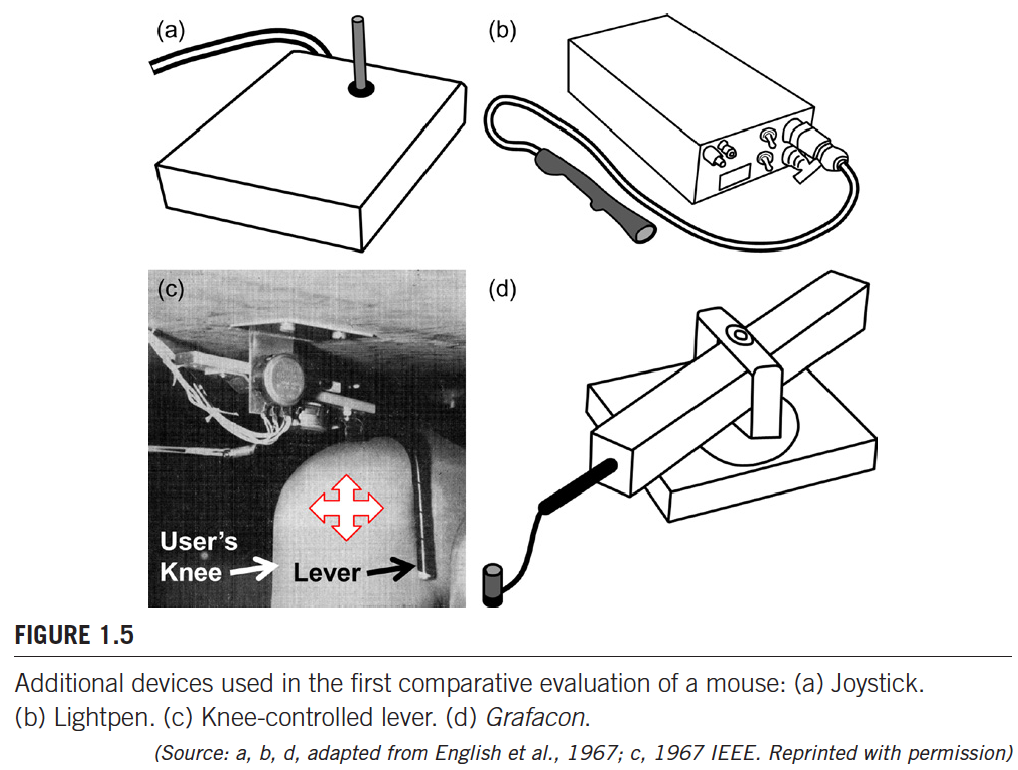
\includegraphics[width=0.6\linewidth]{user-study}
	\caption{Source: Fg 1.5 (Mackenzie)}
\end{figure}
\end{frame}

\begin{frame}
\frametitle{HCI First User Study}
\begin{itemize}
	\item First ever ``user study" %Engelbart conducted the which will later inspire how HCI conducts research
	\item \textbf{Selecting} and \textbf{manipulating} text
	\item Compared \textbf{mouse} with %Engelbart
	\begin{itemize}
		\item \textbf{Light pen} %-  selection at pen barrel, pen pointing directing to the object,
		\item  \textbf{Joystick}% - selection by pressing, moving using stick
		\item \textbf{Knee-controlled lever}% - selection by keyboard, moving by knee movements
		\item \textbf{Grafacon}% - selection by pressing knobs, moving using extensible arms
	\end{itemize}
	\item Three metrics %were used
	\begin{itemize}
		\item \textbf{Access time} - hand from keyboard to device %the time to move the 
		\item \textbf{Motion time} - onset of cursor to the final selection %the time from the 
		\item \textbf{Errors} - distance between center of target and center of cursor
	\end{itemize}
\end{itemize}
\end{frame}

\begin{frame}
\frametitle{HCI First User Study}

\begin{columns}[c] % The "c" option specifies centered vertical alignment while the "t" option is used for top vertical alignment
	
	\column{.4\textwidth} % Left column and width
	\begin{figure}
		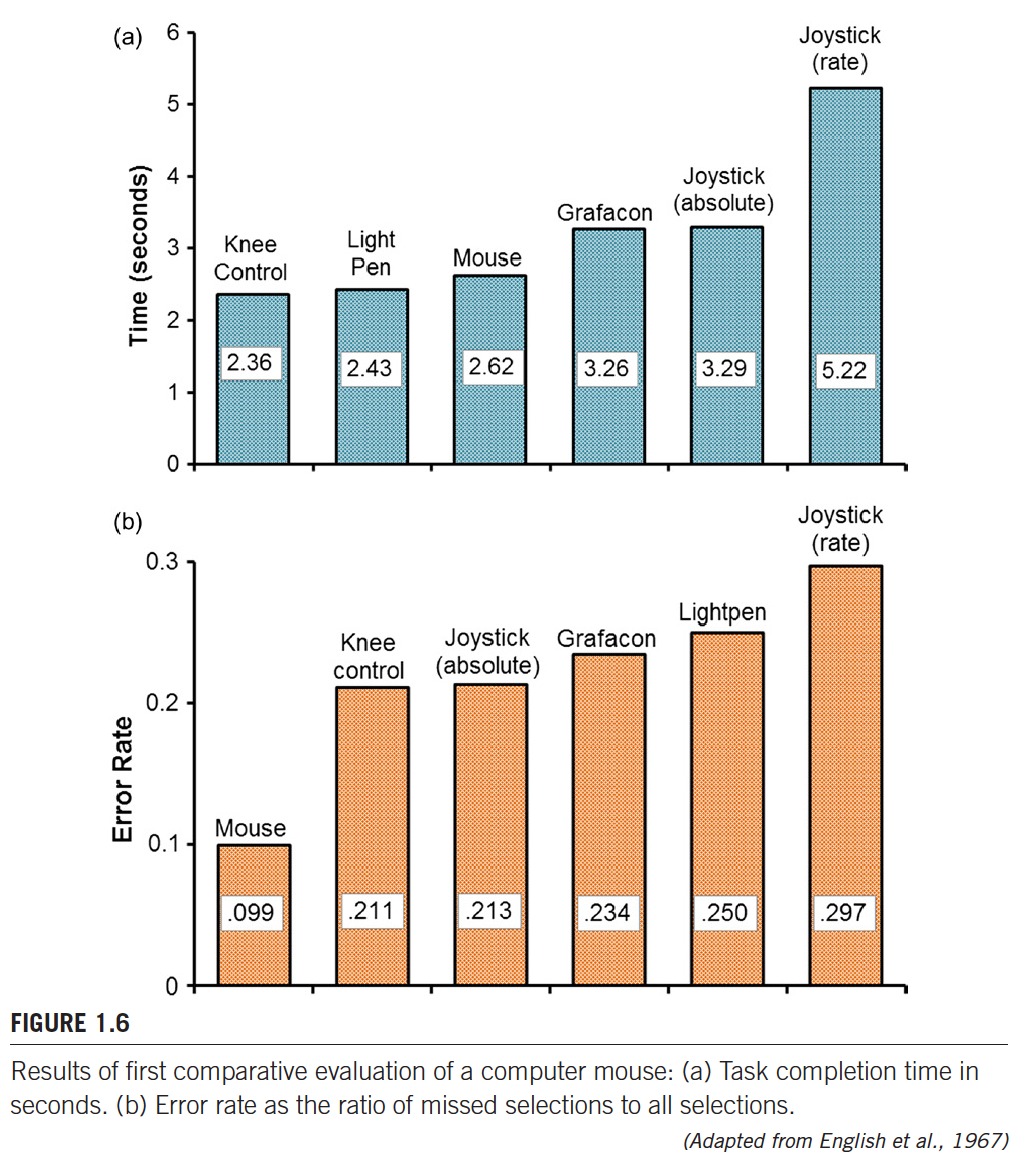
\includegraphics[width=1\linewidth]{results}
		\caption{Source: Fg 1.6 (Mackenzie) - Access time + Motion time = Task Completion time}
	\end{figure}
	
	\column{.6\textwidth} % Right column and width
	\begin{itemize}
		\item 11 participants (8 experienced and 3 inexperienced)
		\item \textbf{A character target at random X and Y pos with varied size appeared}, with surrounding distractors
		\item The trial begin with a spacebar hit, a cursor will appear, and participant move his or her hand to the input device and move the cursor to the target, and make selection
		\item Ten trials / device
	\end{itemize}
	
\end{columns}

\end{frame}

\begin{frame}
\frametitle{HCI First User Study}
\begin{itemize}
	\item Although \textbf{Knee-controlled lever} is best in terms of time, since Knee-controlled has zero access time, the authors argued that considering only motion time, Knee control does not perform well
	\item \textbf{Light pen} performs slightly better than \textbf{mouse}, but because of possible fatigue, mouse will be better in the long run
	\item \textbf{Mouse} is the clear winner in terms of accuracy
\end{itemize}
\end{frame}

\begin{frame}
\frametitle{Discussion}
\begin{itemize}
	\item Why require \textbf{distractors}?
	\item Why require a \textbf{spacebar hit}?
	\item Why require \textbf{10 trials} and not 1 or 2?  How to determine 10?
	\item Why not only measure \textbf{time},  but also \textbf{errors}?
	\item Why a mix of \textbf{experienced} and \textbf{inexperienced}?  and why 11 participants?
	\item How do you choose your \textbf{comparison tools}?  Why light pen or joystick,  for example?  Why command line is not being compared?
	\item Do you think the \textbf{order of factor }matters?  For example,  always do light pen first.
\end{itemize}
\end{frame}

%\begin{frame}
%\frametitle{HCI First User Study}
%\begin{itemize}
%	\item This evaluation marks an important milestone in HCI
%	\begin{itemize}
%		\item Participants
%		\item Apparatus
%		\item Cautious procedure %Detailed description of 
%		\item Input methods $\rightarrow$ \textbf{Independent Variable (IV)}%, with six levels - mouse, light pen, joystick (position-control), joystick (rate-control),  knee controlled lever and Grafacon
%		\item Time and error rate $\rightarrow$ \textbf{Dependent Variables (DV)}
%		\item \textbf{Counterbalancing} procedure %was used %To make sure that there are no order effects, 
%		\item No \textbf{statistical analysis} but is excusable%authors at that time have limited tools at their disposal
%	\end{itemize}
%\end{itemize}
%\end{frame}

%\begin{frame}
%\begin{center} 
%\usebeamerfont*{frametitle} \usebeamercolor[fg]{frametitle}  5-mins break 
%\end{center}
%\end{frame}

%\begin{frame}
%\frametitle{Mouse continue to evolve}
%\begin{itemize}
%	\item Next published evaluation on mouse (Card et al., 1978)
%	\begin{itemize}
%		\item At Xerox PARC
%		\item Part of the larger effort to make the first GUI
%		\item Wheels were replaced with a rolling ball assembly (Rider, 1974)
%	\end{itemize}
%	\item In 1997, Engelbart received the ACM Turing Award (similar to Nobel Prize) and the ACM SIGCHI Lifetime Achievement Award (1998; 1st recipient).   
%	\item Commercialization of mouse starts at 1981, when the Xerox Star was launched
%\end{itemize}
%\end{frame}

\subsection{Xerox Star (1981)} % A subsection can be created just before a set of slides with a common theme to further break down your presentation into chunks

\begin{frame}
\frametitle{At the NCC (1981)}

\begin{columns}[c] % The "c" option specifies centered vertical alignment while the "t" option is used for top vertical alignment
	
	\column{.3\textwidth} % Left column and width
	\begin{figure}
			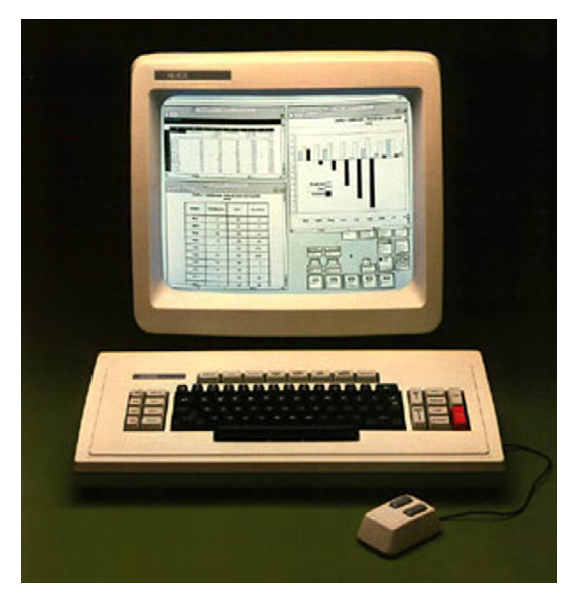
\includegraphics[width=1\linewidth]{xerox}
			\caption{Source: Fg 1.7 (Mackenzie)}
	\end{figure}
	
	\column{.7\textwidth} % Right column and width
	\begin{itemize}
		\item \textbf{National Computer Conference (NCC) }was the yearly conference for computing.  Gathered major players like IBM.   The attendance exceeded 100,000
		\item In May 1981 at NCC, \textbf{Xerox} attracted a lot of buzz regarding their \textbf{Xerox 8100 Star Information System} that supports
		\begin{itemize}
			\item Windows, icons, menus and a pointing device (WIMP)
			\item  Direct manipulation and what-you-see-is-what-you-get (WYSIWYG) interaction
		\end{itemize}	
	\end{itemize}				
\end{columns}
\end{frame}

\begin{frame}
\frametitle{Star}
\url{https://www.youtube.com/watch?v=wOAm7EiFNu8}
\end{frame}


%\begin{frame}
%\frametitle{Journey of the Star}
%\begin{itemize}
%	\item The journey of \textit{Star} began around 1970, when Xerox established its research center, PARC in Palo Alto, CA %and in the following year, signed an agreement with SRI licensing Xerox to use Engelbart's invention.
%	\item \textit{Alto}, the \textit{Star}'s predecessor, began in 1972 and include a GUI and mouse.  Nevertheless, Alto was never released commercially
%	\item  \textit{Star} followed the \textit{Alto}, featuring a novel bit-mapped display, providing rich image (comparing to character-mapped displays), a two-button mouse, and keyboard.  Supports ethernet connection.  Documents, graphic tables, presentations are supported too
%\end{itemize}
%\end{frame}

\begin{frame}
\frametitle{Star's Desktop Metaphor}
\begin{figure}
	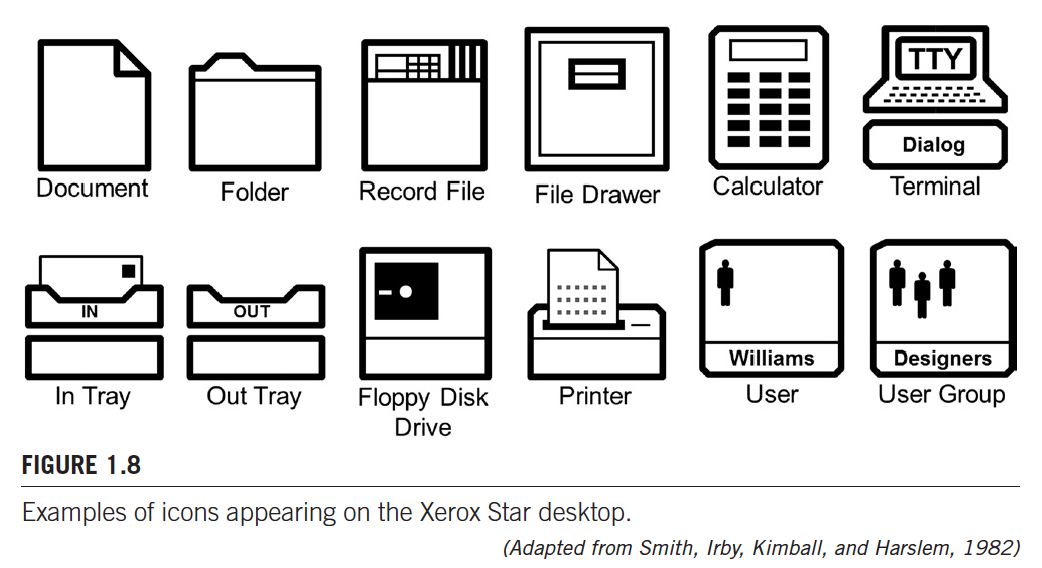
\includegraphics[width=0.5\linewidth]{metaphors}
	\caption{Source: Fg 1.8 (Mackenzie)}
\end{figure}
\begin{itemize}
	\item One novel feature of the Star was the use of \textit{desktop metaphor}
	\item \textbf{Metaphors} are important in HCI.  It allows almost no learning in understanding how to use systems
\end{itemize}
\end{frame}

\begin{frame}
\frametitle{Star's File Systems}
\begin{itemize}
	\item To make the system usable, Star focus on i\textbf{nteractions with files, rather than program}.  Thus, when user clicked a file, the file should automatically open the associated program
	\item All these programs are hidden from the users, thus users are not burdened with lots of programs, but instead, work with the more familiar ``file-system"
\end{itemize}
\end{frame}

\begin{frame}
\frametitle{Star's Direct Manipulation}
\begin{itemize}
	\item Supports point-select interaction
%	\item Previous command-line interfaces had a single channel of input, i.e., specific syntax and commands
	\item Direct manipulation in Star supports \textbf{multiple input channels}, and each channel has a direct correspondent of the task - \textbf{display brightness} or \textbf{sound} use \textit{slider}, \textbf{font size} or \textbf{family} use \textit{menu item}
	\item These direct manipulation channels can be done \textbf{in any order} - giving users the sense of \textbf{control}
	\item To implement direct manipulation, systems shifted from \textit{sequential programming} to \textit{event-driven programming}
\end{itemize}
\end{frame}

\begin{frame}
\frametitle{Star's GUI}
\begin{itemize}
	\item To design GUI, PARC lead by Alan Kay developed a new object-oriented programming language known as \textit{Smalltalk} and a software architecture known as Model-View-Controller
	\item This GUI takes almost 10 years to develop, where a lot of the time was spent on inventing the architecture
\end{itemize}
\end{frame}

\begin{frame}
\frametitle{Star's commercial failure and Apple II}
\begin{itemize}
	\item In the end, Star was not so successful
	\item 3 reasons were identified
	\begin{enumerate}
		\item Star was not really a \textit{personal} computer.  PARC viewed Star as a beefed up version of a terminal connected to a central server.
		\item Star architecture was ``closed" - could only run Xerox applications
		\item Expensive - \$16,000
	\end{enumerate}
	\item Anyhow, the \textit{Apple II}, introduced in 1977, was hugely successful.  The original retail price was \$1,298 featuring the same components as Star and supports 4KB of ram (but without mouse) thus require typing to launch programs
	\begin{itemize}
		\item the platform for VisiCalc, the first spreadsheet application which sells over 700,000 copies and become known as the first ``killer app"
	\end{itemize}
\end{itemize}
\end{frame}

%\begin{frame}
%\frametitle{Other personal computers}
%\begin{itemize}
%	\item Around the same time as Apple II, there were other personal computers include \textit{PET}, \textit{VIC-20}, \textit{Commodore 64}, and \textit{TRS-80}
%	\item However, they were unsuccessful because of their \textbf{terrible} user interface - worked mostly with traditional command-line
%%	\item Operating Systems usually consisted of BASIC-language interpreter and a console prompt.  LOAD, SAVE, RUN, EDIT and few other commands were about it.
%	\item Technical users love these systems but that's it.  These systems did not go far.
%\end{itemize}
%\end{frame}

%\begin{frame}
%\begin{center} 
%\usebeamerfont*{frametitle} \usebeamercolor[fg]{frametitle}  5-mins break 
%\end{center}
%\end{frame}

\subsection{Birth of HCI (1983)} % A subsection can be created just before a set of slides with a common theme to further break down your presentation into chunks

\begin{frame}
\frametitle{Birth of HCI (1983)}
\begin{itemize}
	\item 1983 was possibly among the most notable milestone of HCI and were defined by three important feats: 
	\begin{enumerate}
		\item the first \textbf{ACM SIGCHI conference}
		\item publication of Card, Moran, and Newell's \textit{The Psychology of Human Computer Interaction (1983)}
		\item arrival of \textbf{Apple Macintosh} in January 1984
	\end{enumerate}
\end{itemize}
\end{frame}

%\begin{frame}
%\frametitle{First ACM SIGCHI Conference (1983)}
%\begin{itemize}
%	\item HCI roots reach as early as 1969, when ACM's \textit{Special Interest Group on Social and Behavioral Computing (SIGSOC)} was formed
%	\item SIGSOC focused on computers in the social sciences, however, the emphasis shifted to user needs
%	\item In 1978, SIGSOC lobbied for a name change and was eventually change to SIGCHI - \textit{Conference on Human Factors in Computing Systems}
%	\item SIGCHI's mission defined as follows where the interdisplinary nature was evident: \textit{This interdisciplinary group is composed of computer scientists, software engineers, psychologists, interaction designers, graphic designers, sociologists, and anthropologists...brought together by a shared understanding that designing useful and usable technology is an interdisciplinary process, and believe....(can) transform persons' lives.}
%\end{itemize}
%\end{frame}

\begin{frame}
\frametitle{(1) First ACM SIGCHI Conference (1983)}
\begin{figure}
	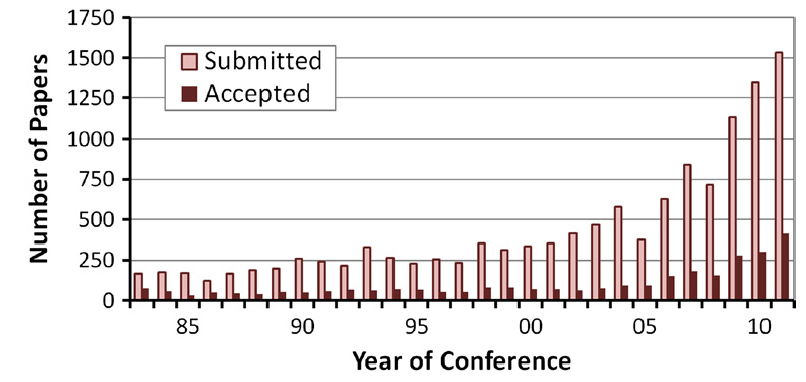
\includegraphics[width=0.5\linewidth]{submissions}
	\caption{Source: Fg 1.9 (Mackenzie)}
\end{figure}
\footnotesize
\begin{itemize}
	\item The \textbf{first SIGCHI conference} was held in Boston with 59 technical papers presentations.  
	\item Since then, SIGCHI is widely known as CHI (k sound) and has attendance of about 4,000
	\item CHI publication has since becomes the standard of HCI academia
%	\item Research papers in CHI is peer-reviewed and competitive.  Statistics from 1982 to 2011 indicate a total of 12,671 paper submissions with 3,018 acceptances, for an overall acceptance rate of 24 percent.
\end{itemize}
\end{frame}

%\begin{frame}
%\frametitle{(1) First ACM SIGCHI Conference (1983)}
%\begin{itemize}
%	\item CHI papers usually have \textbf{high visibility}, and thus has a tendency to have \textbf{high citations}
%	\item In contrast to other fields, CHI proceedings are much \textbf{more valuable} than most HCI journals
%%	\item Feel free to check the impact at \textbf{Google Scholar h5-index} in the field of HCI (search ``google scholar HCI")
%	\item Along the way, there were establishments of other venues, including tier-1 journals for HCI - \textit{TOCHI (ACM)}, \textit{HCI} (Taylor and Francis) and tier-1 conferences such as \textit{User Interface Software and Technology} (UIST)
%\end{itemize}
%\end{frame}

\begin{frame}
\frametitle{(2) The Psychology of Human-Computer Interaction (1983)}
\begin{itemize}
	\item Card and Moran arrived at PARC in 1974 and seek to \textbf{apply the knowledge of human sensory, cognitive and motor systems to HCI}. 
	\item This knowledge was eye-opening where  \textit{Model Human Processor} (MHP) was proposed
	\item The MHP had an \textbf{eye} and a \textbf{ear} (for sensory input to a perceptual processor), a \textbf{brain} (with a cognitive processor, short-term memory, and long-term memory), and an \textbf{arm}, \textbf{hand}, and \textbf{finger} (for motor responses) 
	\item MHP is the first to show that \textbf{human can be modeled}
\end{itemize}
\end{frame}

\begin{frame}
\frametitle{Model Human Processor}
\begin{figure}
	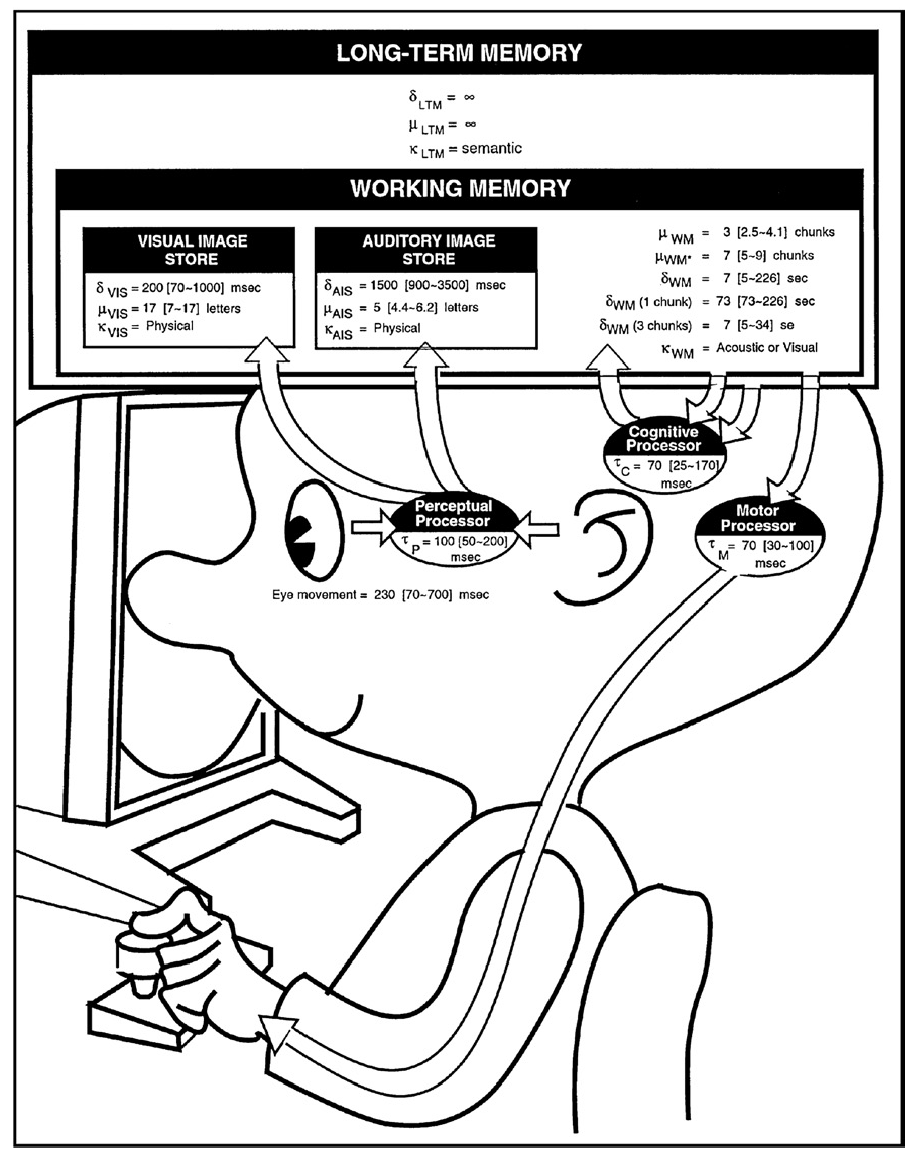
\includegraphics[width=0.4\linewidth]{mhp}
	\caption{Source: Fg 1.11 (Mackenzie)}
\end{figure}
\end{frame}

%
%\begin{frame}
%\footnotesize
%\frametitle{The use of MHP}
%\begin{itemize}
%	\item For example, \textit{suppose a user types "hello" on some predictive text-entry system (T9).  After entering 4(GHI), 3(DEF), 5(JKL), 5(JKL), 6(MNO), a word appears on the display.  If the word matches what the user wants, he select the word.  If isn't, he swipe to next word.  What is the task completion time between signal and response for the matching case?} (Card et al., 1983, p. 66)
%	\item We can \textbf{use MHP to model the task completion} time, Here there are four low-level processing cycles: a perceptual processor cycle \textit{$ t_{p} $} (look at the word), two cognitive processor cycles \textit{$ t_{c} $} (think whether it matches, and then have decided it's a yes) and a motor processor cycle \textit{$ t_{m} $} (tell the hand to select).  For each value, it is bracketed by an expected minimum and maximum, where these values were obtained through basic research.
%\end{itemize}
%\begin{figure}
%	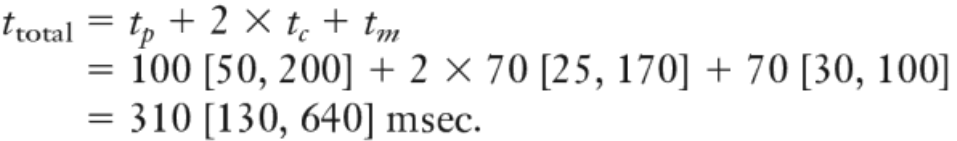
\includegraphics[width=0.7\linewidth]{mhptime2}
%\end{figure}
%\end{frame}

%\begin{frame}
%\frametitle{HCI models}
%\begin{itemize}
%	\item Other prominent models of human behaviors include \textbf{keystroke-level model} (KLM), \textbf{goals, operators, methods, and selection rules models} (GOMS),  \textbf{Hick's law for choice reaction time} (Hick, 1952)and \textbf{Fitts' law for rapid aimed movement} (Fitts, 1954).
%%	\item Model is powerful because it allows a better understanding of \textbf{relationships} (descriptive models) or a \textbf{quantitative prediction} (predictive models). 
%	\item Current research is about using these models as \textbf{cost functions} for optimizations in deep learning
%\end{itemize}
%\end{frame}

\begin{frame}
\frametitle{(3) Launch of the Apple Macintosh (1984)}
\begin{figure}
	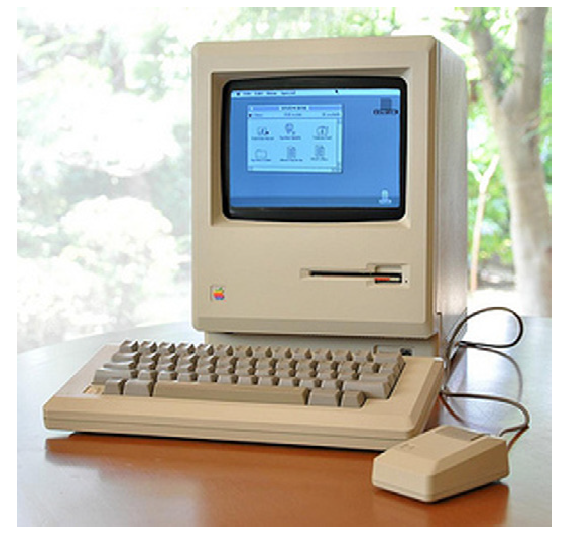
\includegraphics[width=0.5\linewidth]{mac2}
	\caption{Source: Fg 1.12 (Mackenzie)}
	\url{https://www.youtube.com/watch?v=3vq9p00T08I}
\end{figure}
\end{frame}

\begin{frame}
\frametitle{Launch of the Apple Macintosh (1984)}
\begin{itemize}
	\item Apple Macintosh was launched in January 22, 1984, selling at \$2,495.  Sold 70,000 unit by May 3, 1984
	\item Introducing \textbf{one-button mouse}
	\item Used MacOS - \textbf{icons-based}
	\item Featured 128KB Ram, and for storage, it introduced \textbf{3.5 inch disks} that stored 400K (later 800K then 1.44MB), enough to store application
	\item Bundled with System, Finder, MacPaint, MacWrite, MacProject, MacTerminal, and Microsoft Word
\end{itemize}
\end{frame}

\subsection{Graphical User Interfaces (GUI)} % A subsection can be created just before a set of slides with a common theme to further break down your presentation into chunks

\begin{frame}
\frametitle{Growth of HCI and GUIs}
\begin{itemize}
	\item Microsoft was a latecomer in GUIs.  Early version of Microsoft \textit{Windows} appeared in 1985, but it was not until \textit{Windows 3.0} (1990) and \textit{Windows 3.1} (1992) that Microsoft became a real threat to Mac
	\item Major \textbf{universities} offered courses in HCI
	\item \textbf{Companies} also paid great effort in their HCI departments
	\item \textbf{SIGCHI conferences} remain the main driver
\end{itemize}
\end{frame}

\subsection{HCI Research} % A subsection can be created just before a set of slides with a common theme to further break down your presentation into chunks

%\begin{frame}
%\frametitle{Growth of HCI research}
%\begin{itemize}
%	\item Research interests in HCI was about \textbf{quality}, \textbf{effectiveness}, and \textbf{efficiency} of the interface.  How \textbf{accurately} and \textbf{quickly} can people do common tasks using a GUI vs. command-line interface?  Given two implementations of GUI, which one is \textbf{quicker} or \textbf{accurate}?
%	\item Empirical research (also known as formal approach) are commonly used.  \textbf{Qualitative/Heuristic} evaluation are also used but are often debated how ``objective'' these methods are, and how it depends on ones' interpretations rather than on factual measurements.  \textbf{Bio-signals metrics} are proposed as alternative for more objective measurement of emotions, cognitions, and behaviors
%\end{itemize}
%\end{frame}

\begin{frame}
\frametitle{Early Days HCI research}
\begin{itemize}
	\item A classic example of early days is on the \textbf{design of menus.}
	\begin{itemize}
		\item \textbf{Speed}: \textit{Marking menus} - \url{https://www.youtube.com/watch?v=dtH9GdFSQaw}
		\item \textbf{Order}: How menu items should be ordered?  Alphabetically or by function?
		\item \textbf{Metaphor}: Is access improve if an icon is added to the label?
		\item \textbf{Depth vs. Breadth}: Go deeper or wider?
		\item \textbf{Organization}: Which menu to put "Indent Text"?
	\end{itemize}
	\item \textbf{Spirit of HCI research} is similar to above questions %Although most of these answers were addressed, 
\end{itemize}
\end{frame}

\subsection{Resources} % A subsection can be created just before a set of slides with a common theme to further break down your presentation into chunks

\begin{frame}
\frametitle{Online Resources}
\begin{itemize}
	\item ACM Digital Library - \url{http://dl.acm.org}
	\item HCI pioneers - \url{https://hcipioneers.wordpress.com/}
	\item ACM Interactions - \url{http://interactions.acm.org/}
	\item HCI Bibliography - \url{http://www.hcibib.org/}
	\item Textbook - \url{http://www.yorku.ca/mack/HCIbook/}
	\item  Human Computer Interaction - \textbf{Brief Intro by John Caroll}, \url{https://www.interaction-design.org/literature/book/the-encyclopedia-of-human-computer-interaction-2nd-ed/human-computer-interaction-brief-intro}  
\end{itemize}
\end{frame}

\begin{frame}
\frametitle{What's next}
Read my slide on \textbf{Empirical} and these textbook resources:
\begin{itemize}
	\item Mackenzie, Chapter 4-5, \textbf{Scientific Foundations, Designing HCI Experiments},  Human Computer Interaction: An Empirical Research Perspective, 1st ed. (2013) 
	\item Zhao, \textbf{How to Design Controlled Experiments in HCI?} \url{https://www.slideshare.net/shilman/controlled-experiments-shengdong-zhao}\
\end{itemize}
\end{frame}

%\begin{frame}
%\frametitle{Assignment (Individual)}
%Access the homework via Google Classroom (code found at the intro slide)
%	\begin{figure}
%		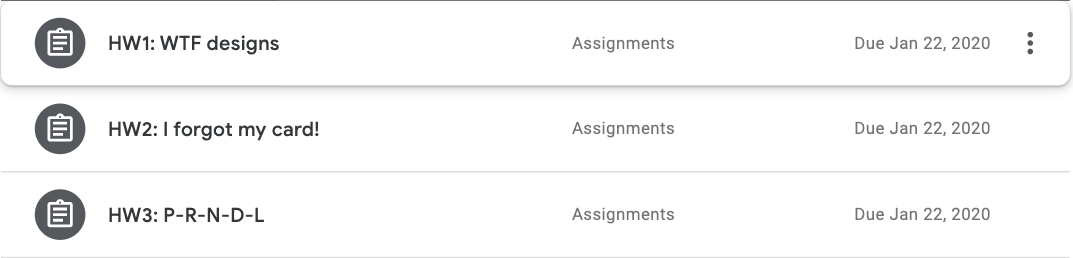
\includegraphics[width=1\linewidth]{assignment}
%	\end{figure}
%\end{frame}

%\section{What's next}
%
%\begin{frame}
%\frametitle{What's next}
%Read my slide on \textbf{BCI}.
%\end{frame}

\begin{frame}
\Huge{\centerline{Questions}}
\end{frame}

%----------------------------------------------------------------------------------------

\end{document} 